\documentclass{article}
\usepackage[utf8]{inputenc}
\usepackage{amssymb,amsmath}
\usepackage[parfill]{parskip}
\DeclareMathOperator*{\argmin}{arg\,min}
\DeclareMathOperator*{\argmax}{arg\,max}
\usepackage{graphicx}
\usepackage{subcaption}

\usepackage{mathtools}
\DeclareMathOperator{\tr}{tr}

\title{Optimization 10/36-725\\
        Homework 2}
\author{Willie Neiswanger}
\date{}

\begin{document}

\maketitle


\section{Problem Five}

\begin{figure}[h!tbp]
        \center{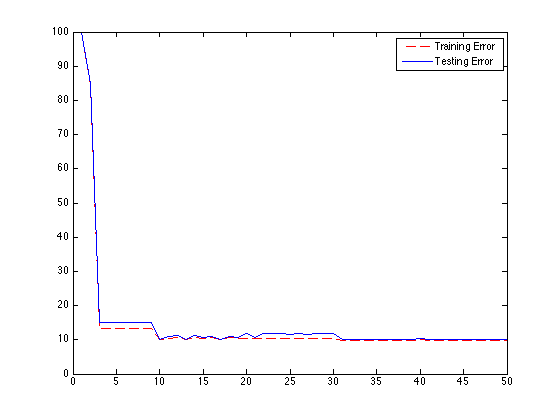
\includegraphics[width=0.5\textwidth]{img/p5_bt.png}}
       \caption{Gradient boosting with back tracking line search ($\gamma_1=0.5, \gamma_2=0.5$).}
\end{figure}

\begin{figure}[h!tbp]
        \center{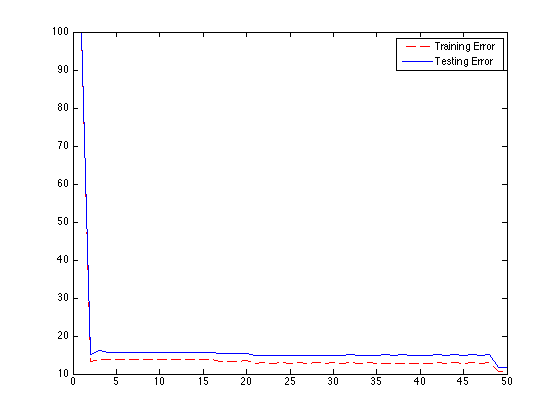
\includegraphics[width=0.5\textwidth]{img/p5_bt2.png}}
       \caption{Gradient boosting with back tracking line search ($\gamma_1=0.1, \gamma_2=0.5$).}
\end{figure}

\begin{figure}[h!tbp]
        \center{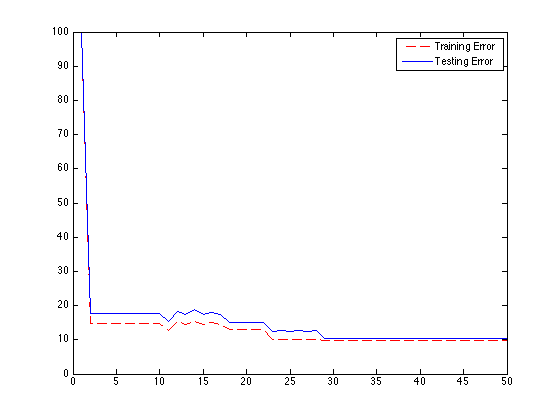
\includegraphics[width=0.5\textwidth]{img/p5_bt3.png}}
       \caption{Gradient boosting with back tracking line search ($\gamma_1=0.1, \gamma_2=0.1$).}
\end{figure}

\begin{figure}[h!tbp]
        \center{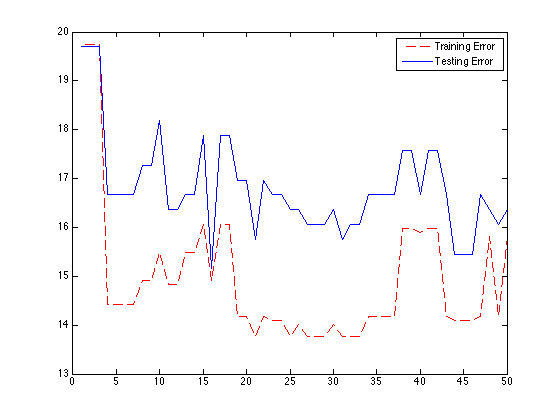
\includegraphics[width=0.5\textwidth]{img/p5_fixed1.png}}
       \caption{Gradient boosting with fixed step size ($\alpha=0.1$).}
\end{figure}

\begin{figure}[h!tbp]
        \center{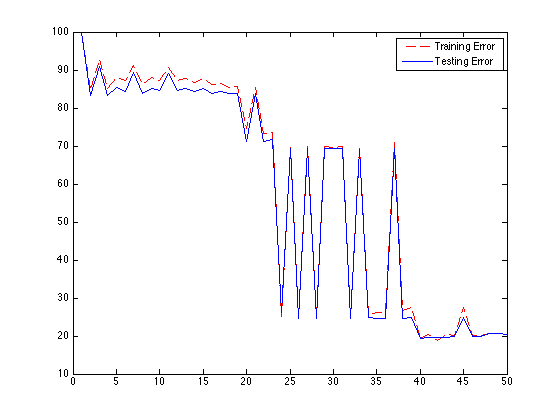
\includegraphics[width=0.5\textwidth]{img/p5_fixed2.png}}
       \caption{Gradient boosting with fixed step size ($\alpha=0.5$).}
\end{figure}

\newpage
It seems that the backtracking strategy is able to make a few large jumps early
on and then remain at a good (low) objective value for the remaining
iterations, while the fixed step-size travels in a more consistent and smooth
manner towards a lower objective value. In all cases, the testing errors seems
to be highly correlated with the training error, but is in general higher than
the training error (as we would expect).

\end{document}
